\documentclass{article}

\usepackage{arxiv}
\usepackage{graphicx}
\usepackage[utf8]{inputenc} % allow utf-8 input
\usepackage[T1]{fontenc}    % use 8-bit T1 fonts
\usepackage{hyperref}       % hyperlinks
\usepackage{url}            % simple URL typesetting
\usepackage{booktabs}       % professional-quality tables
\usepackage{amsfonts}       % blackboard math symbols
\usepackage{nicefrac}       % compact symbols for 1/2, etc.
\usepackage{microtype}      % microtypography
\usepackage{lipsum}

\title{SPI}


\author{SebastianOsorio , Sergio Vargas, Robison Steven} \\
  %% \AND
  %% Coauthor \\
  %% Affiliation \\
  %% Address \\
  %% \texttt{email} \\
  %% \And
  %% Coauthor \\
  %% Affiliation \\
  %% Address \\
  %% \texttt{email} \\
  %% \And
  %% Coauthor \\
  %% Affiliation \\
  %% Address \\
  %% \texttt{email} \\
}

\begin{document}
\maketitle 


\keywords{MISO, MOSI,  Sclk,  CS}

Se desea crear un protocolo de comunicación que sea capaz de comunicarse con un acelerómetro, para esto las siguientes especificaciones.

El protocolo SPI master que se implementa tendrá cuatro cables los cuales serán MISO, MOSI, sclk , CS, Dout y además también tendrá un reloj de entrada clk. Este protoco esta diseñado para comunicarse con un acelerómetro ADXL362, el cual funciona con una polaridad cero $(POL=0)$ y uns fase cero $(PHA=0)$, es decir que nuestro maestro tendrá que emplear el flanco de bajada. 



\subsection{clk} Es el reloj trasmitido por la FPGA($100\ MHz$), el cual debe llegar a una librería capas de disminuir la frecuencia y distribuirla por otra salida.
\subsection{Miso} Se debe usar para una comunicación serial, donde el acelerómetro se comunicara con el protocolo spi.
\subsection{Mosi} Se debe usar para una comunicación del protocolo spi al acelerómetro de forma serial. Este canal es empleado para trasmitir las instrucciones $(Escritura\ 0X0A\ y\ lectura\ 0X0B)$  y las direcciones $(registro_x\ 0X0F,\ registro_y\ 0X11\ y \ registro_y\ 0X13)$respectivamente en este orden, cada una de un byte.

Las instrucciones empleadas 
\subsection{CS} Es una linea de habilitación de puerto serie y esta controlada por el maestro spi, en donde el estado bajo significa el comienzo de la trasmisión  acelerómetro y el modo alto finaliza la  trasmisión, este $CS$ corresponde al que el maestro SPI envía al acelerómetro.

\subsection{Dout} Es el dato almacenado por la comunicación con miso, este dato debe ser de 8 bit, el llevara la información del dada del acelerómetro al protocolo spi y del protocolo spi a una memoria. 

\subsection{Sclk} Se emplea para sincronizar la comunicación que para el caso del acelerómetro debe ser tener una frecuencia menor a $8\ MHz$.

\subsection{Memoria} Se debe usar una memoria que se comunique con el protocolo spi y esta también sea capaz de enviar datos a los demás protocolos, debe tener las siguientes especificaciones.

tener una entrada en paralelo de 8 bit, la cual debe ser enviada por el protocolo de comunicación spi, este dato debe ser comparado, ya que es el que se utiliza para informar si el acelerómetro esta en movimiento.
tener una salida, la cual de una señal que alerte si el acelerómetro a tenido movimientos no normales que puedan ser señal de inseguridad.

\subsection{Descripción}
El periférico inicia la comunicación escribiendo en el acelerómetro 

\section{Protocolo de comunicacion SPI}

En general, se realizo una maquina de estados sincrona para determinar los procesos que se realizan en tiempos especificos de cilcos de relog. Los modulos usados fueron tres: El divisor de frecuencias para establecer la frecuencia a la que la transmicion se lleva a cabo, el contador para establecer una sincronizacion de los procesos al enviar y recibir datos del acelerometro y la maquina de estados que define que se debe enviar o leer en tiempos especificos. 

Las variables que se comparten con el acelerometros son: MOSI (salida de datos del maestra hacia el acelerometro), MISO (entrada de datos del acelerometro al maestro), cs (inicializacion y finalizacion de la comunicacion con el esclavo) y sclk para sincronizar los datos de entrada y salida.

\subsection{Divisor}

Para bajar la frecuencia del relog de la Nexys se uso el registro "count" de 14 bits.

Para generar un relog a partir de dicha variable se empieza a sumar 1 al valor actual (empezando en 0) en referencia al flanco de subida del relog, luego se asigna el relog de salida como el bit mas significativo de "count". La frecuencia de salida es:

\begin{center}
    \[ f_{sclk}=\frac{f_{in}}{2^{14}}=\]
\end{center}

\subsection{Contador}

El contador es un modulo que consta de un registro de 5 bits, se usa hasta llegar a un conteo de 26 (numero de ciclos de sclk a los cuales ya se terminaron de realizar los procesos necesarios para enviar informacion, recibir una respuesta de esta y luego cargar los datos del registro a una salida.

\subsection{Maquina de estados}

Este modulo es el mas importante del codigo, debido a que decodifica y realiza los estados sincronamente. Los estados se realizan en flanco de bajada o subida de relog, segun sea escritura de MOSI (bajada) o lectura de MISO (subida). Existen 4 estados.

Los siguientes estados se reailzan en flanco de bajada:

\subsection{Din_charge}

El estado de carga de dato asigna a los 8 bits mas significativos del registro "shift-mo" el valor de la instruccion (se encuentra fija en lectura simple), para los siguientes 8 bits carga al registro la direccion que se quiere leer del acelerometro.

\subsection{MO_sh}

Este estado lee el registro "shift-mo" desde el bit mas significativo hasta completar todo el registro.

\subsection{MI-sh}

Para flanco de subida, al llegar a este estado se reinicia MOSI dejandolo en 1 (estado natural cuando no esta enviando datos).

\subsection{Dout-charge}

Cuando se completa la lectura de MISO, se cambia al estado de carga donde el registro "shift-mi" pasa a ser el dato de salida "Dout".

Los siguientes estadosse realizan en flanco de subida:

\subsection{MI-sh}

Este estado en flanco de subida, se realiza para leer los datos que llegan de miso(del acelerometro hacia el maestro) desde el bit más significativo, hasta completar todo el registro.

\section{Diagrama}

\begin{figure}[H]

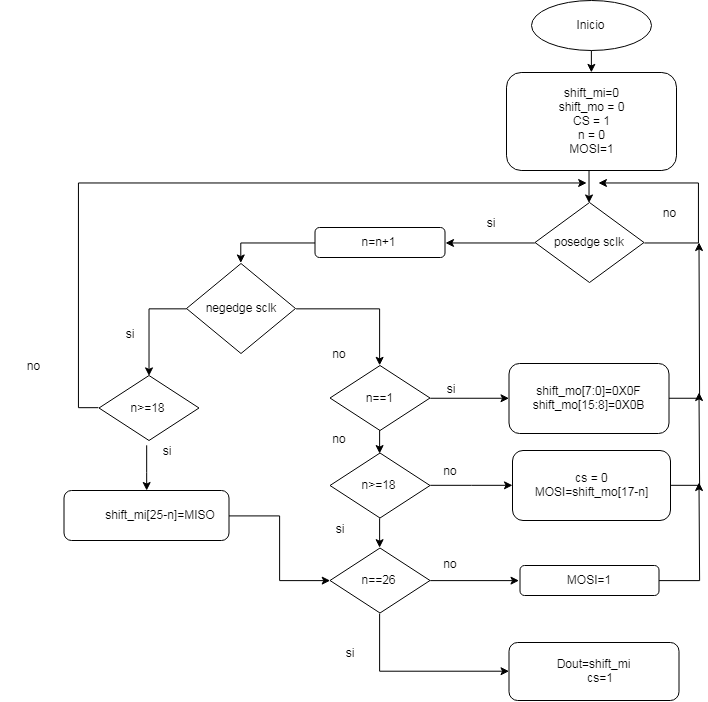
\includegraphics[scale=0.5]{3.png}
\caption{diagrama funcional spi}
\label{imagen 1}
\end{figure}

\begin{figure}[H]
\centering
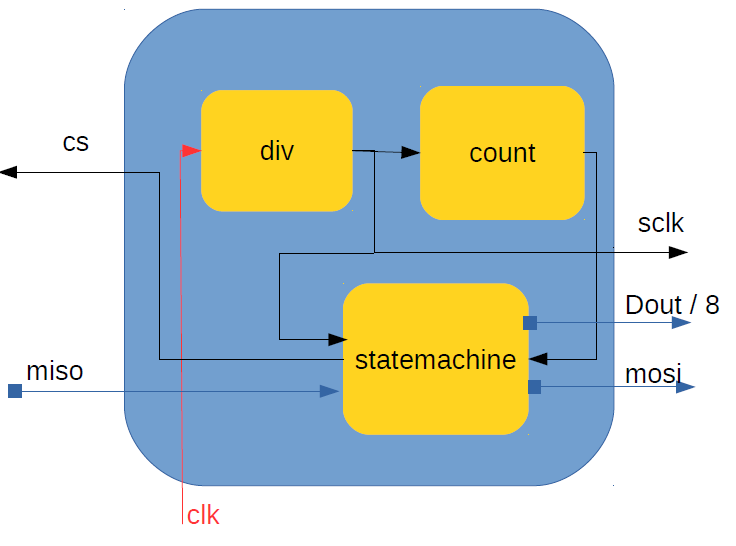
\includegraphics[scale=0.5]{d2.PNG}
\caption{Caja Negra}
\label{imagen 1}
\end{figure}


\begin{figure}[H]
\centering
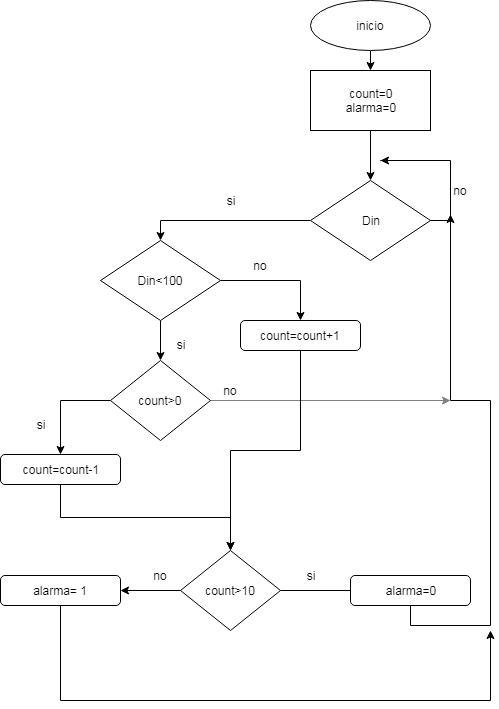
\includegraphics[scale=0.5]{D.png}
\caption{diagrama funcional con memoria}
\label{imagen 1}
\end{figure}

\begin{figure}[H]
\centering
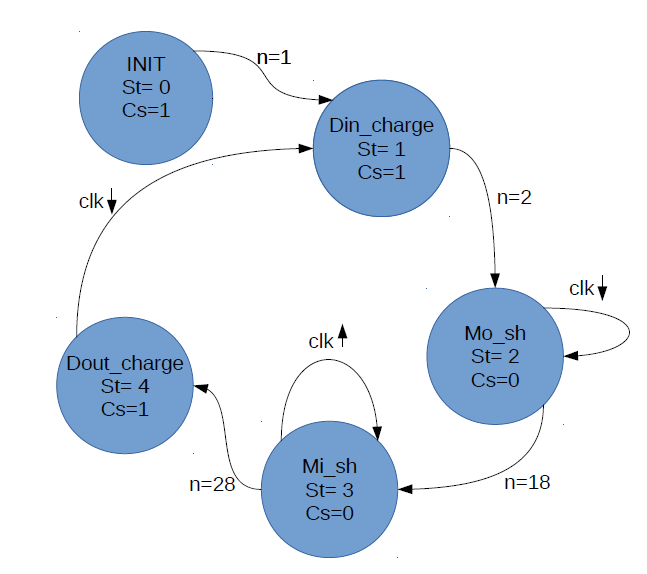
\includegraphics[scale=0.65]{d1.PNG}
\caption{Diagrama de estados}
\label{imagen 1}
\end{figure}



\begin{figure}[H]

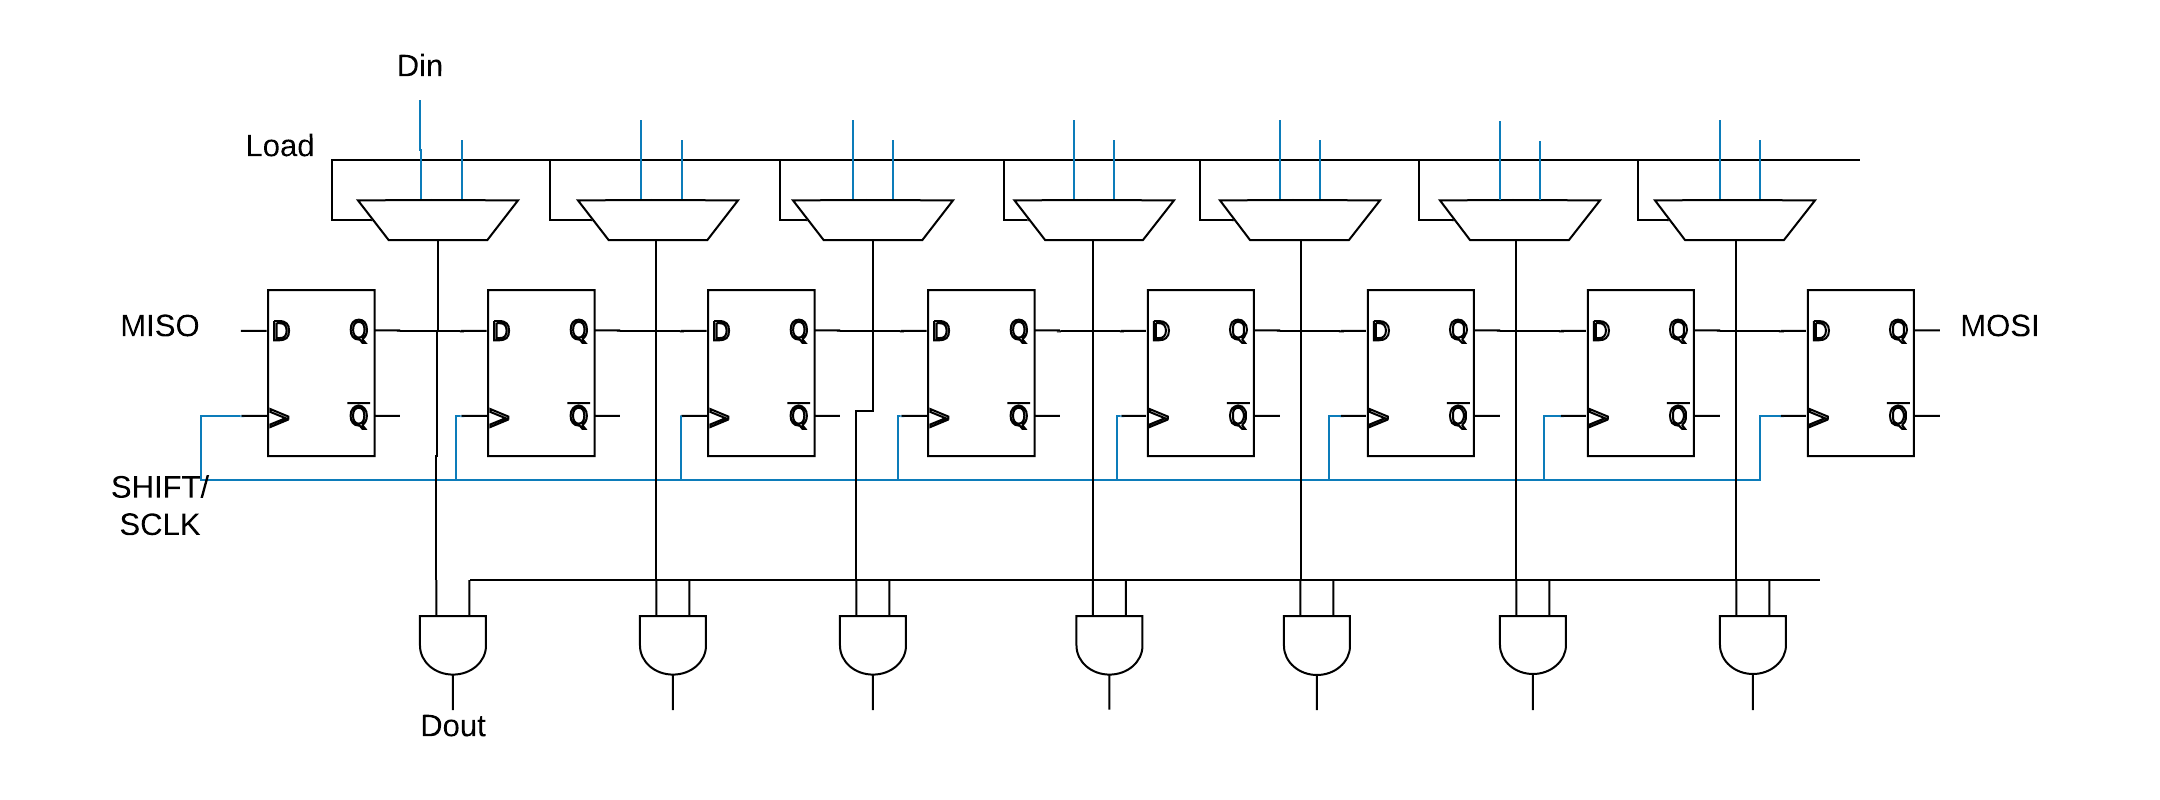
\includegraphics[scale=0.5]{1.png}
\caption{Registro de desplazamiento}
\label{imagen 1}
\end{figure}

\begin{figure}[H]

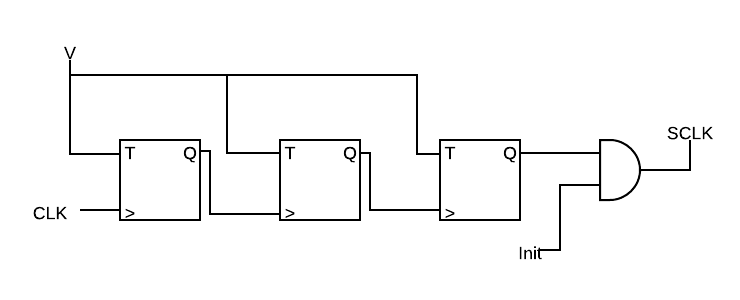
\includegraphics[scale=1]{DIV.png}
\caption{Divisor}
\label{imagen 1}
\end{figure}


















%\bibliography{references}  %%% Remove comment to use the external .bib file (using bibtex).
%%% and comment out the ``thebibliography'' section.


%%% Comment out this section when you \bibliography{references} is enabled.



\end{document}
